\documentclass{extbook}[14pt]
\usepackage{multicol, enumerate, enumitem, hyperref, color, soul, setspace, parskip, fancyhdr, amssymb, amsthm, amsmath, bbm, latexsym, units, mathtools}
\everymath{\displaystyle}
\usepackage[headsep=0.5cm,headheight=0cm, left=1 in,right= 1 in,top= 1 in,bottom= 1 in]{geometry}
\usepackage{dashrule}  % Package to use the command below to create lines between items
\newcommand{\litem}[1]{\item #1

\rule{\textwidth}{0.4pt}}
\pagestyle{fancy}
\lhead{}
\chead{Answer Key for Progress Quiz 4 Version A}
\rhead{}
\lfoot{8448-1521}
\cfoot{}
\rfoot{Fall 2020}
\begin{document}
\textbf{This key should allow you to understand why you choose the option you did (beyond just getting a question right or wrong). \href{https://xronos.clas.ufl.edu/mac1105spring2020/courseDescriptionAndMisc/Exams/LearningFromResults}{More instructions on how to use this key can be found here}.}

\textbf{If you have a suggestion to make the keys better, \href{https://forms.gle/CZkbZmPbC9XALEE88}{please fill out the short survey here}.}

\textit{Note: This key is auto-generated and may contain issues and/or errors. The keys are reviewed after each exam to ensure grading is done accurately. If there are issues (like duplicate options), they are noted in the offline gradebook. The keys are a work-in-progress to give students as many resources to improve as possible.}

\rule{\textwidth}{0.4pt}

\begin{enumerate}\litem{
Which of the following equations \textit{could} be of the graph presented below?

\begin{center}
    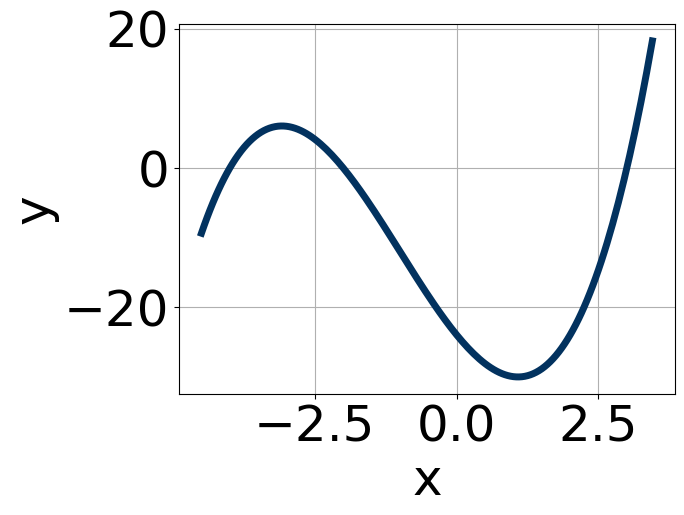
\includegraphics[width=0.5\textwidth]{../Figures/polyGraphToFunctionCopyA.png}
\end{center}



The solution is \( -5(x + 2)^{6} (x - 1)^{4} (x + 3)^{10} \), which is option E.\begin{enumerate}[label=\Alph*.]
\item \( -5(x + 2)^{6} (x - 1)^{8} (x + 3)^{11} \)

The factor $(x + 3)$ should have an even power.
\item \( 12(x + 2)^{6} (x - 1)^{10} (x + 3)^{5} \)

The factor $(x + 3)$ should have an even power and the leading coefficient should be the opposite sign.
\item \( 7(x + 2)^{10} (x - 1)^{10} (x + 3)^{8} \)

This corresponds to the leading coefficient being the opposite value than it should be.
\item \( -7(x + 2)^{6} (x - 1)^{7} (x + 3)^{7} \)

The factors $(x - 1)$ and $(x + 3)$ should both have even powers.
\item \( -5(x + 2)^{6} (x - 1)^{4} (x + 3)^{10} \)

* This is the correct option.
\end{enumerate}

\textbf{General Comment:} General Comments: Draw the x-axis to determine which zeros are touching (and so have even multiplicity) or cross (and have odd multiplicity).
}
\litem{
Construct the lowest-degree polynomial given the zeros below. Then, choose the intervals that contain the coefficients of the polynomial in the form $x^3+bx^2+cx+d$.
\[ 2 + 5 i \text{ and } -4 \]
The solution is \( x^{3} +13 x + 116 \), which is option C.\begin{enumerate}[label=\Alph*.]
\item \( b \in [0.16, 1.34], c \in [0, 5], \text{ and } d \in [-9, -3] \)

$x^{3} + x^{2} +2 x -8$, which corresponds to multiplying out $(x -2)(x + 4)$.
\item \( b \in [-1.51, 0.14], c \in [4, 21], \text{ and } d \in [-119, -107] \)

$x^{3} +13 x -116$, which corresponds to multiplying out $(x-(2 + 5 i))(x-(2 - 5 i))(x -4)$.
\item \( b \in [-1.51, 0.14], c \in [4, 21], \text{ and } d \in [112, 121] \)

* $x^{3} +13 x + 116$, which is the correct option.
\item \( b \in [0.16, 1.34], c \in [-2, 0], \text{ and } d \in [-20, -14] \)

$x^{3} + x^{2} -x -20$, which corresponds to multiplying out $(x -5)(x + 4)$.
\item \( \text{None of the above.} \)

This corresponds to making an unanticipated error or not understanding how to use nonreal complex numbers to create the lowest-degree polynomial. If you chose this and are not sure what you did wrong, please contact the coordinator for help.
\end{enumerate}

\textbf{General Comment:} Remember that the conjugate of $a+bi$ is $a-bi$. Since these zeros always come in pairs, we need to multiply out $(x-(2 + 5 i))(x-(2 - 5 i))(x-(-4))$.
}
\litem{
Which of the following equations \textit{could} be of the graph presented below?

\begin{center}
    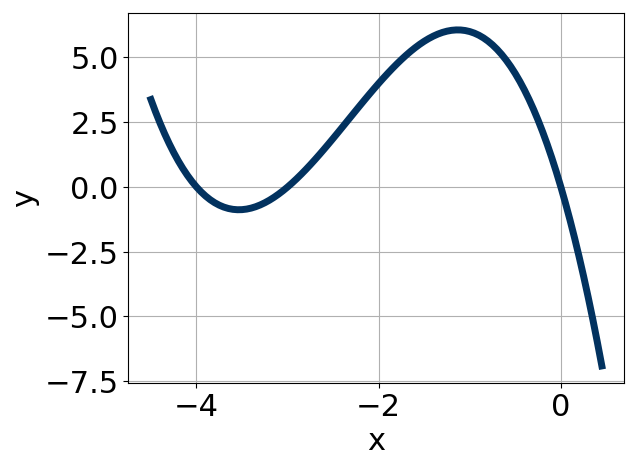
\includegraphics[width=0.5\textwidth]{../Figures/polyGraphToFunctionA.png}
\end{center}



The solution is \( -16x^{10} (x + 2)^{5} (x - 1)^{5} \), which is option A.\begin{enumerate}[label=\Alph*.]
\item \( -16x^{10} (x + 2)^{5} (x - 1)^{5} \)

* This is the correct option.
\item \( -14x^{10} (x + 2)^{8} (x - 1)^{7} \)

The factor $(x + 2)$ should have an odd power.
\item \( -15x^{5} (x + 2)^{4} (x - 1)^{9} \)

The factor $0$ should have an even power and the factor $-2$ should have an odd power.
\item \( 8x^{4} (x + 2)^{11} (x - 1)^{8} \)

The factor $(x - 1)$ should have an odd power and the leading coefficient should be the opposite sign.
\item \( 2x^{4} (x + 2)^{5} (x - 1)^{11} \)

This corresponds to the leading coefficient being the opposite value than it should be.
\end{enumerate}

\textbf{General Comment:} General Comments: Draw the x-axis to determine which zeros are touching (and so have even multiplicity) or cross (and have odd multiplicity).
}
\litem{
Describe the zero behavior of the zero $x = -3$ of the polynomial below.
\[ f(x) = -3(x + 3)^{2}(x - 3)^{5}(x + 4)^{9}(x - 4)^{10} \]
The solution is the graph below, which is option C.
\begin{center}
    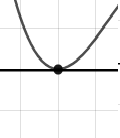
\includegraphics[width=0.3\textwidth]{../Figures/polyZeroBehaviorCA.png}
\end{center}\begin{enumerate}[label=\Alph*.]
\begin{multicols}{2}
\item 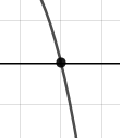
\includegraphics[width = 0.3\textwidth]{../Figures/polyZeroBehaviorAA.png}
\item 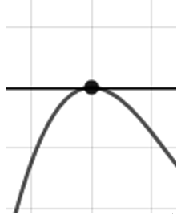
\includegraphics[width = 0.3\textwidth]{../Figures/polyZeroBehaviorBA.png}
\item 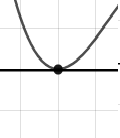
\includegraphics[width = 0.3\textwidth]{../Figures/polyZeroBehaviorCA.png}
\item 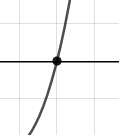
\includegraphics[width = 0.3\textwidth]{../Figures/polyZeroBehaviorDA.png}
\end{multicols}\item None of the above.\end{enumerate}
\textbf{General Comment:} You will need to sketch the entire graph, then zoom in on the zero the question asks about.
}
\litem{
Describe the zero behavior of the zero $x = 5$ of the polynomial below.
\[ f(x) = 9(x + 5)^{5}(x - 5)^{10}(x + 7)^{9}(x - 7)^{12} \]
The solution is the graph below, which is option C.
\begin{center}
    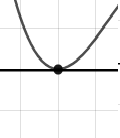
\includegraphics[width=0.3\textwidth]{../Figures/polyZeroBehaviorCopyCA.png}
\end{center}\begin{enumerate}[label=\Alph*.]
\begin{multicols}{2}
\item 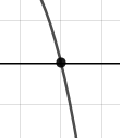
\includegraphics[width = 0.3\textwidth]{../Figures/polyZeroBehaviorCopyAA.png}
\item 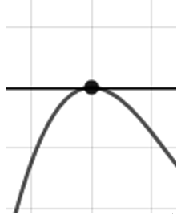
\includegraphics[width = 0.3\textwidth]{../Figures/polyZeroBehaviorCopyBA.png}
\item 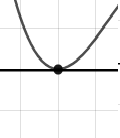
\includegraphics[width = 0.3\textwidth]{../Figures/polyZeroBehaviorCopyCA.png}
\item 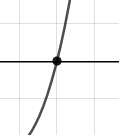
\includegraphics[width = 0.3\textwidth]{../Figures/polyZeroBehaviorCopyDA.png}
\end{multicols}\item None of the above.\end{enumerate}
\textbf{General Comment:} You will need to sketch the entire graph, then zoom in on the zero the question asks about.
}
\litem{
Describe the end behavior of the polynomial below.
\[ f(x) = 9(x - 4)^{4}(x + 4)^{9}(x - 6)^{4}(x + 6)^{4} \]
The solution is the graph below, which is option D.
\begin{center}
    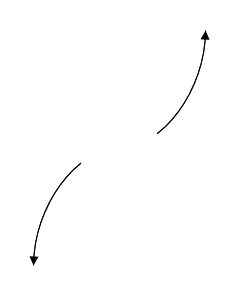
\includegraphics[width=0.3\textwidth]{../Figures/polyEndBehaviorCopyDA.png}
\end{center}\begin{enumerate}[label=\Alph*.]
\begin{multicols}{2}
\item 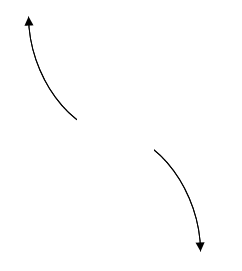
\includegraphics[width = 0.3\textwidth]{../Figures/polyEndBehaviorCopyAA.png}
\item 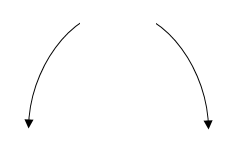
\includegraphics[width = 0.3\textwidth]{../Figures/polyEndBehaviorCopyBA.png}
\item 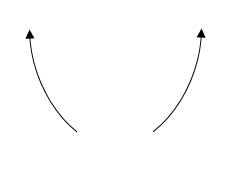
\includegraphics[width = 0.3\textwidth]{../Figures/polyEndBehaviorCopyCA.png}
\item 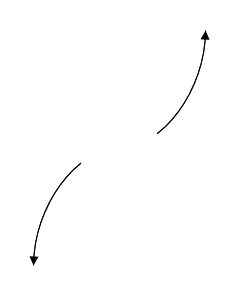
\includegraphics[width = 0.3\textwidth]{../Figures/polyEndBehaviorCopyDA.png}
\end{multicols}\item None of the above.\end{enumerate}
\textbf{General Comment:} Remember that end behavior is determined by the leading coefficient AND whether the \textbf{sum} of the multiplicities is positive or negative.
}
\litem{
Describe the end behavior of the polynomial below.
\[ f(x) = -9(x - 9)^{2}(x + 9)^{3}(x - 4)^{2}(x + 4)^{4} \]
The solution is the graph below, which is option A.
\begin{center}
    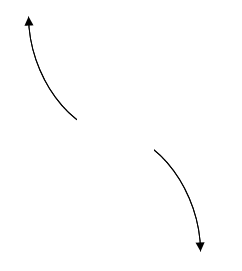
\includegraphics[width=0.3\textwidth]{../Figures/polyEndBehaviorAA.png}
\end{center}\begin{enumerate}[label=\Alph*.]
\begin{multicols}{2}
\item 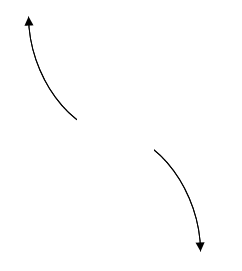
\includegraphics[width = 0.3\textwidth]{../Figures/polyEndBehaviorAA.png}
\item 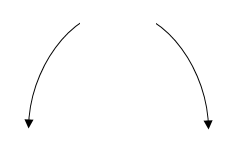
\includegraphics[width = 0.3\textwidth]{../Figures/polyEndBehaviorBA.png}
\item 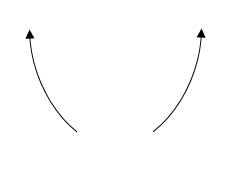
\includegraphics[width = 0.3\textwidth]{../Figures/polyEndBehaviorCA.png}
\item 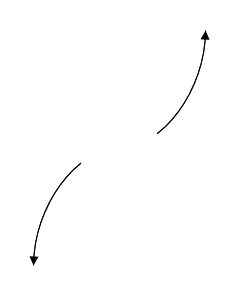
\includegraphics[width = 0.3\textwidth]{../Figures/polyEndBehaviorDA.png}
\end{multicols}\item None of the above.\end{enumerate}
\textbf{General Comment:} Remember that end behavior is determined by the leading coefficient AND whether the \textbf{sum} of the multiplicities is positive or negative.
}
\litem{
Construct the lowest-degree polynomial given the zeros below. Then, choose the intervals that contain the coefficients of the polynomial in the form $ax^3+bx^2+cx+d$.
\[ \frac{-2}{5}, \frac{3}{5}, \text{ and } \frac{2}{3} \]
The solution is \( 75x^{3} -65 x^{2} -8 x + 12 \), which is option C.\begin{enumerate}[label=\Alph*.]
\item \( a \in [74, 76], b \in [58, 66], c \in [-12, -2], \text{ and } d \in [-18, -4] \)

$75x^{3} +65 x^{2} -8 x -12$, which corresponds to multiplying out $(5x -2)(5x + 3)(3x + 2)$.
\item \( a \in [74, 76], b \in [-36, -34], c \in [-30, -26], \text{ and } d \in [12, 17] \)

$75x^{3} -35 x^{2} -28 x + 12$, which corresponds to multiplying out $(5x + 5)(5x + 5)(3x -3)$.
\item \( a \in [74, 76], b \in [-70, -60], c \in [-12, -2], \text{ and } d \in [12, 17] \)

* $75x^{3} -65 x^{2} -8 x + 12$, which is the correct option.
\item \( a \in [74, 76], b \in [-129, -119], c \in [61, 70], \text{ and } d \in [-18, -4] \)

$75x^{3} -125 x^{2} +68 x -12$, which corresponds to multiplying out $(5x + 5)(5x -5)(3x -3)$.
\item \( a \in [74, 76], b \in [-70, -60], c \in [-12, -2], \text{ and } d \in [-18, -4] \)

$75x^{3} -65 x^{2} -8 x -12$, which corresponds to multiplying everything correctly except the constant term.
\end{enumerate}

\textbf{General Comment:} To construct the lowest-degree polynomial, you want to multiply out $(5x + 2)(5x -3)(3x -2)$
}
\litem{
Construct the lowest-degree polynomial given the zeros below. Then, choose the intervals that contain the coefficients of the polynomial in the form $ax^3+bx^2+cx+d$.
\[ \frac{-7}{5}, \frac{3}{4}, \text{ and } \frac{-3}{2} \]
The solution is \( 40x^{3} +86 x^{2} -3 x -63 \), which is option B.\begin{enumerate}[label=\Alph*.]
\item \( a \in [40, 44], b \in [-92, -83], c \in [-5, 1], \text{ and } d \in [59, 64] \)

$40x^{3} -86 x^{2} -3 x + 63$, which corresponds to multiplying out $(5x -7)(4x + 3)(2x -3)$.
\item \( a \in [40, 44], b \in [85, 87], c \in [-5, 1], \text{ and } d \in [-67, -58] \)

* $40x^{3} +86 x^{2} -3 x -63$, which is the correct option.
\item \( a \in [40, 44], b \in [30, 40], c \in [-84, -78], \text{ and } d \in [-67, -58] \)

$40x^{3} +34 x^{2} -81 x -63$, which corresponds to multiplying out $(5x + 5)(4x + 4)(2x -2)$.
\item \( a \in [40, 44], b \in [-27, -22], c \in [-87, -82], \text{ and } d \in [59, 64] \)

$40x^{3} -26 x^{2} -87 x + 63$, which corresponds to multiplying out $(5x + 5)(4x -4)(2x -2)$.
\item \( a \in [40, 44], b \in [85, 87], c \in [-5, 1], \text{ and } d \in [59, 64] \)

$40x^{3} +86 x^{2} -3 x + 63$, which corresponds to multiplying everything correctly except the constant term.
\end{enumerate}

\textbf{General Comment:} To construct the lowest-degree polynomial, you want to multiply out $(5x + 7)(4x -3)(2x + 3)$
}
\litem{
Construct the lowest-degree polynomial given the zeros below. Then, choose the intervals that contain the coefficients of the polynomial in the form $x^3+bx^2+cx+d$.
\[ 3 - 5 i \text{ and } 3 \]
The solution is \( x^{3} -9 x^{2} +52 x -102 \), which is option A.\begin{enumerate}[label=\Alph*.]
\item \( b \in [-14, -5], c \in [51, 58], \text{ and } d \in [-109, -97] \)

* $x^{3} -9 x^{2} +52 x -102$, which is the correct option.
\item \( b \in [4, 16], c \in [51, 58], \text{ and } d \in [99, 103] \)

$x^{3} +9 x^{2} +52 x + 102$, which corresponds to multiplying out $(x-(3 - 5 i))(x-(3 + 5 i))(x + 3)$.
\item \( b \in [-1, 4], c \in [1, 3], \text{ and } d \in [-17, -10] \)

$x^{3} + x^{2} +2 x -15$, which corresponds to multiplying out $(x + 5)(x -3)$.
\item \( b \in [-1, 4], c \in [-19, -3], \text{ and } d \in [5, 11] \)

$x^{3} + x^{2} -6 x + 9$, which corresponds to multiplying out $(x -3)(x -3)$.
\item \( \text{None of the above.} \)

This corresponds to making an unanticipated error or not understanding how to use nonreal complex numbers to create the lowest-degree polynomial. If you chose this and are not sure what you did wrong, please contact the coordinator for help.
\end{enumerate}

\textbf{General Comment:} Remember that the conjugate of $a+bi$ is $a-bi$. Since these zeros always come in pairs, we need to multiply out $(x-(3 - 5 i))(x-(3 + 5 i))(x-(3))$.
}
\end{enumerate}

\end{document}